% ============================================================
%  Figure 6 — Condition number comparison: Stage 1 vs Seq. Est.
%  Bar chart with fault types on x-axis
% ============================================================
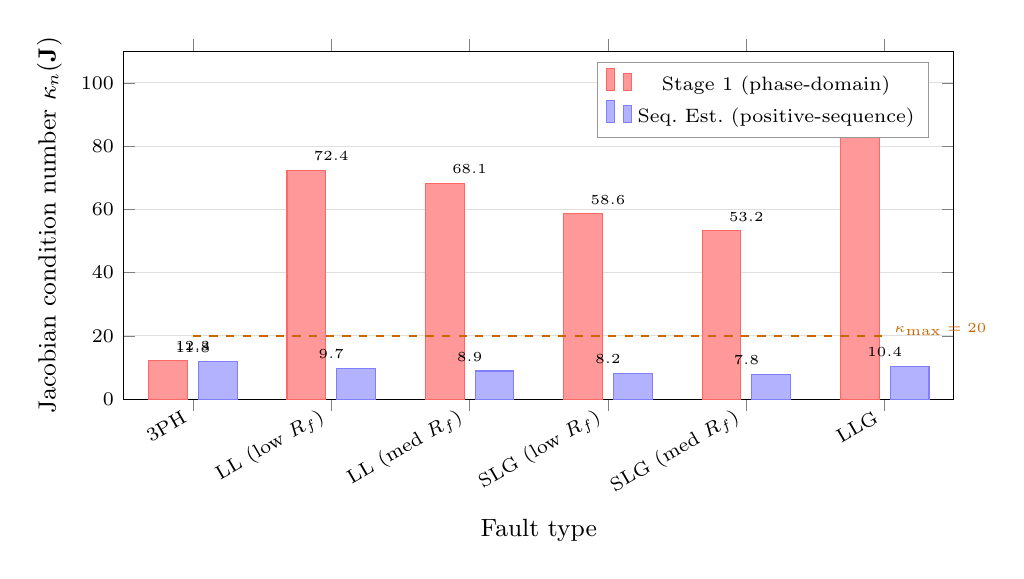
\begin{tikzpicture}
\begin{axis}[
  width=\columnwidth, height=6.0cm,
  ybar=4pt,
  bar width=14pt,
  xlabel={Fault type},
  ylabel={Jacobian condition number $\kappa_n(\mathbf{J})$},
  symbolic x coords={3PH, LL (low $R_f$), LL (med $R_f$), SLG (low $R_f$), SLG (med $R_f$), LLG},
  xtick=data,
  x tick label style={rotate=30, anchor=east, font=\scriptsize},
  ymin=0, ymax=110,
  ytick={0,20,40,60,80,100},
  ymajorgrids=true, grid style={gray!25},
  label style={font=\small},
  tick label style={font=\scriptsize},
  legend style={at={(0.97,0.97)}, anchor=north east,
                font=\scriptsize, fill=white, draw=black!40},
  nodes near coords,
  nodes near coords align={vertical},
  every node near coord/.style={font=\tiny},
  clip=false
]

% Stage 1 (phase-domain) condition numbers
\addplot[fill=red!40, draw=red!60] coordinates {
  (3PH,                12.3)
  (LL (low $R_f$),     72.4)
  (LL (med $R_f$),     68.1)
  (SLG (low $R_f$),    58.6)
  (SLG (med $R_f$),    53.2)
  (LLG,                88.2)
};

% Sequence estimator (positive-sequence only) condition numbers
\addplot[fill=blue!30, draw=blue!50] coordinates {
  (3PH,                11.8)
  (LL (low $R_f$),      9.7)
  (LL (med $R_f$),      8.9)
  (SLG (low $R_f$),     8.2)
  (SLG (med $R_f$),     7.8)
  (LLG,                10.4)
};

% Threshold line — use a ybar-safe approach: draw as extra bar at y=20
\draw[thick, orange!80!black, dashed]
  ({axis cs:3PH,0}|-{axis cs:3PH,20}) --
  ({axis cs:LLG,0}|-{axis cs:LLG,20});
\node[right, font=\tiny, orange!80!black]
  at (axis cs:{LLG},22) {$\kappa_{\max}=20$};

\legend{Stage~1 (phase-domain),
        Seq.\ Est.\ (positive-sequence)};
\end{axis}
\end{tikzpicture}
